\clearpage
\begingroup
\fancyhead[R]{\sffamily\small\color{Muted}Vulkan / 细线抗锯齿}
\setlength{\parindent}{2\ccwd}
\ctexset{section/afterindent=true,subsection/afterindent=true}
\section{一个像素里的细线}

铁丝只遮住像素的四分之一时，这个像素应该同时带有铁丝和背景的颜色。只在中心取一次样，只能得到其中一种。把镜头挪一点，中心刚好越过铁丝，屏幕上就少了一截线。时间抗锯齿（TAA）让每帧的采样位置稍有不同。假设铁丝和背景的光照稳定，16 次采样有 4 次落到铁丝上，线性光照的均值就是四分之一的铁丝颜色，加四分之三的背景颜色。曝光和显示转换在这之后进行。

\begin{center}
\begin{tikzpicture}[x=3.0cm,y=3.0cm]
  \fill[Soft] (0,0) rectangle (1,1);
  \fill[Rust!68] (0,.25) rectangle (1,.5);
  \draw[Rule] (0,0) rectangle (1,1);
  \foreach \x/\y in {9/9,7/5,5/10,12/7,3/6,10/13,13/11,11/3,6/14,8/1,4/2,2/12,0/8,15/4,14/15,1/0}{
    \fill[Ink] ({(\x+.5)/16},{(\y+.5)/16}) circle[radius=.6mm];}
  \node[anchor=west,text=Ink] at (1.10,.69) {一个方格代表一个屏幕像素};
  \node[anchor=west,text=Rust] at (1.10,.43) {红带代表宽度为四分之一像素的细线};
  \node[anchor=west,text=Ink] at (1.10,.17) {16 个点中的 4 个落在红带上};
\end{tikzpicture}
\end{center}

取样点的位置也会影响结果。我们让一条直线从不同方向穿过方格，用它与方格相交的精确面积作对照。测试覆盖 180 个方向、385 个位置，以及 0.2、0.5、1 和 1.5 像素四种线宽。下表只统计部分被线遮住的像素。误差 0.04 表示估计的覆盖面积平均相差整个像素的四个百分点。

{\smalltable\noindent\begin{tabularx}{\linewidth}{@{}Xrr@{}}\toprule
采样方式 & 各方向平均误差 & 误差最大的方向与数值\\\midrule
原版 Halton 序列 & 0.03990 & $45^\circ$，0.05478\\
规则斜排的试验序列 & 0.03069 & $45^\circ$，0.08034\\
将 Vulkan 的 16 个标准点移到小格中心 & 0.02960 & $117^\circ$，0.03801\\
第二组再旋转 $90^\circ$，共 32 个位置 & 0.01888 & $77^\circ$，0.02366\\\bottomrule
\end{tabularx}\par}

旧版固定镜头最多绘制 32 帧，其中后 16 帧重复了前面的采样位置。规则斜排在中庭吊绳的方向表现很好，换成 $45^\circ$ 却比旧版更容易漏采。第三组取自 Vulkan 规范的 16 样点表，每点沿两轴平移 $1/32$ 个像素，让整组的平均位置位于像素中心。第二轮把图案旋转 $90^\circ$，同样的 32 帧便能检查 32 个不同的位置。表中按面积计算，各点等权；实际编辑器的亮度还取决于材质和光照。

\readings{\href{run:../../tests/check_taa_directions.py}{解析面积与各方向的误差}\quad
\refitem{https://docs.vulkan.org/spec/latest/chapters/primsrast.html\#primsrast-standardsamplelocations}{Khronos 标准采样位置}\quad
\refitem{https://pbr-book.org/4ed/Sampling_and_Reconstruction/Stratified_Sampler}{PBRT 第四版第 8.5 节}}

\clearpage
\section{屋顶吊绳的光照与轮廓}

先让 Vulkan 只画 Sponza 的绳子。暂时用纯白表示绳子，用黑色表示空处，相机向一侧缓慢移动。几何阶段的输出已经出现白线时断时续的现象。查原模型也能看到绳段之间有间隔；放大画面检查轮廓时，应该保留这样的空隙。为了量出绘制产生的误差，我们逐个投影三角形，将每个像素细分为 $32\times32$ 个位置，统计其中多少确实落在绳上。

在 $600\times385$ 的画面中，实际光栅器依次绘制了 17 个机位。只在中心取样时，上、下两段绳的边缘覆盖误差分别为 0.213 和 0.227。每个像素同时取 $2\times2$ 个位置后，误差降至 0.068 和 0.076。把前后两张图的覆盖变化与相同机位的参考比较，误差也从 0.101、0.088 降到 0.075、0.072。这里量的是几何面积，还没有计算表面颜色。

\begin{figure}[H]\centering
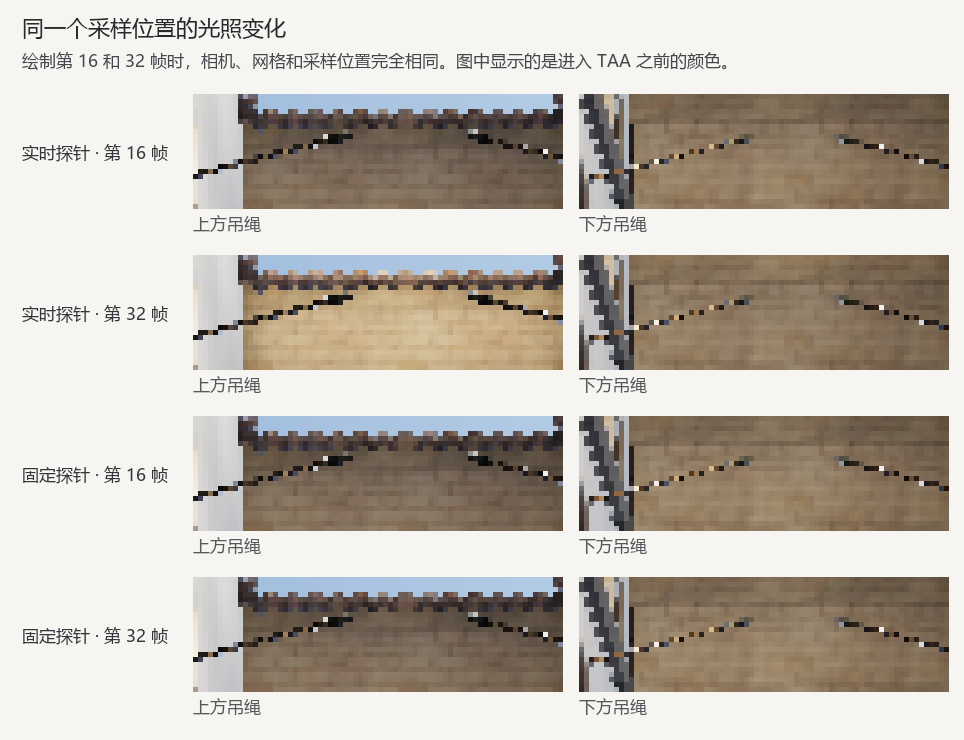
\includegraphics[width=.89\linewidth]{../../../output/validation/atrium-aa/lighting-change.png}
\caption{恢复完整材质后的 RenderDoc 实拍。原版每 16 帧重复一组采样点。左栏的实时光照明显改变，下两行读取同一份已烘焙的光照。图中是颜色送入 TAA 前的结果。}
\end{figure}

对着上方同一排像素比较第 16 帧和第 32 帧。两帧的相机、采到的表面及材质数据逐值相同，但实时 DDGI 还在更新周围的间接光。进入 TAA 前，上方吊绳附近的线性亮度平均增加 0.078。固定使用同一份烘焙探针后，同一批像素的差值为零。判断抗锯齿时先固定照明，再恢复实时探针检查游戏中的画面，可以分清线条的形状和墙面逐渐变亮这两种变化。

\readings{\href{run:../validation/atrium-aa/gpu-pan-coverage.json}{17 个机位的 Vulkan 覆盖实测}\quad
\href{run:../validation/atrium-aa/lighting.json}{对应帧、相机和亮度读数}}

\clearpage
\section{第 32 帧的画面和耗时}

\begin{figure}[H]\centering
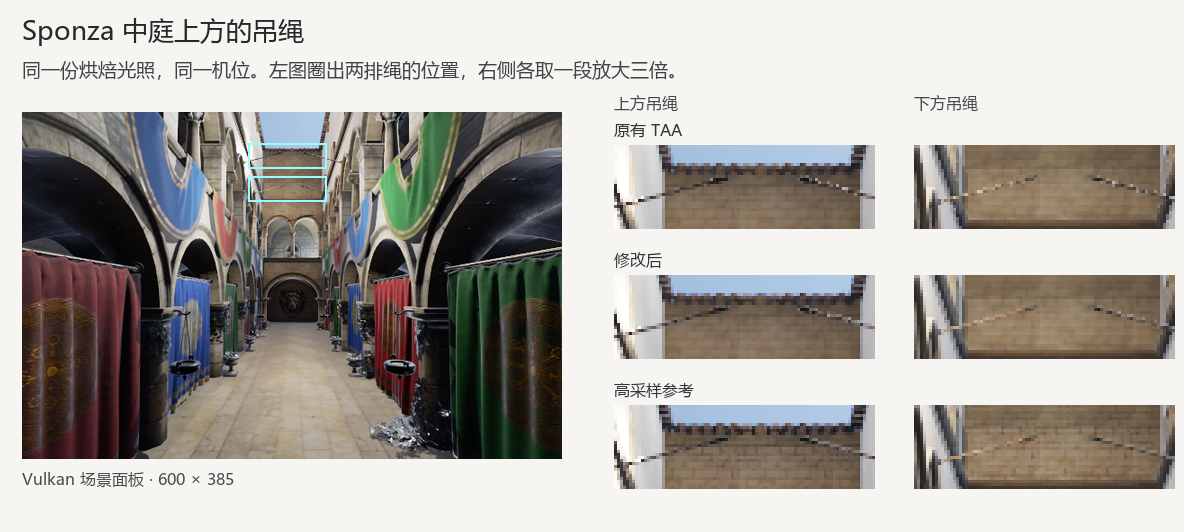
\includegraphics[width=.84\linewidth]{../../../output/validation/atrium-aa/final-wires.png}
\caption{Vulkan 编辑器读回的场景图。三行共享相同机位、材质、曝光和烘焙探针。右下两段绳仍留有原模型的间隔。}
\end{figure}

把面板固定在 $600\times385$，另用 $2400\times1540$ 的画幅取参考。先平均 32 帧在线性空间算出的光，再将高分辨率的每 $4\times4$ 个像素平均成一个面板像素，最后按相同的曝光映射到显示器。沿绳中心上下各取约两个像素，比较显示亮度（0 到 1）。固定光照时，上绳的平均绝对误差由 0.03792 降到 0.03486，下绳由 0.03843 降到 0.02779。实时探针下，与整个采样期间的均值相比，两处从 0.07211、0.03881 降至 0.05827、0.02819。若更看重最近几帧的光照，原生面板上新版的上绳偏暗，下绳仍较接近参考。比较实时画面的报告需要说清参考图取的是哪段时间。

固定镜头时，一个像素在前后两次采样中可能一回落在线上，另一回落在墙上。引擎在已有的表面位置记录中标记这种情况。以后混合这个像素的颜色时，按实际采样次数求均值。移动镜头后，一份旧位置只描述一层表面，这种已经混有两层颜色的记录会被舍弃。另用两根交叉细线连续平移，帧与帧之间的覆盖变化误差从 0.409 降至 0.362，单帧的覆盖误差为 0.285 和 0.288。移动中仍有可能一帧采不到细线。

在 RTX 5070 Ti Laptop 上用 RenderDoc 1.47 回放 Debug 版的第 32 帧。两版各有 228 次绘制和 11 次计算调度。两轮回放交换新旧先后，每次进场预热一次再测六次。下表列出每版 12 个样本的中位数，单位为毫秒。总和包含界面绘制，GPU 等待和显示器呈现另计。

{\smalltable\noindent\begin{tabularx}{\linewidth}{@{}Xrrrr@{}}\toprule
面板尺寸 & 旧 TAA & 新 TAA & 旧绘制和计算 & 新绘制和计算\\\midrule
$600\times385$ & 0.016 & 0.036 & 3.82 & 4.67\\
$1391\times892$ & 0.212 & 0.361 & 11.46 & 13.56\\\bottomrule
\end{tabularx}\par}

两组原生总用时的中间八成样本分别落在 10.97--13.41 ms 和 11.25--15.95 ms。单看 TAA 的增量约为 0.15 ms。CPU 的现有计时段包含等待 Vulkan 围栏的时间，无法从中分出纯提交开销。若要同时降低移动中的误差与显存带宽开销，下一步可以只在存在多层几何的像素增加空间采样，再复用以上两类测量。

\readings{\href{run:../validation/atrium-aa/README.md}{场景、截图与复现入口}\quad
\href{run:../validation/atrium-aa/gpu-final-native.json}{原生面板逐次 GPU 用时}\quad
\refitem{https://research.nvidia.com/labs/rtr/publication/yang2020survey/}{Yang 等人的 TAA 综述}}
\endgroup
